\documentclass{beamer}

\usepackage{amsmath}
\usepackage{graphicx}
\usepackage{tikz}
\usetikzlibrary{positioning}  % ← Add this
\usepackage{pgfplots}
\usepackage{algorithm}
\usepackage{algorithmic}
\usepackage{bm}
\usepackage{url}
\usepackage{listings}
\usepackage{xcolor}
\usepackage{booktabs}
\usepackage{amssymb}  % For \checkmark
\usepackage{pifont}   % For \ding symbols
\newcommand{\cmark}{\ding{51}}  % ✓
\newcommand{\xmark}{\ding{55}}  % ✗

% Configure listings for Python
\lstset{
  language=Python,
  basicstyle=\ttfamily\footnotesize,
  keywordstyle=\color{blue},
  commentstyle=\color{green!50!black},
  stringstyle=\color{red},
  showstringspaces=false,
  breaklines=true,
  frame=single,
  numbers=left,
  numberstyle=\tiny\color{gray},
}

\newcommand{\x}{\mathbf{x}}
\newcommand{\y}{\mathbf{y}}
\newcommand{\z}{\mathbf{z}}
\newcommand{\w}{\mathbf{w}}
\newcommand{\bmu}{\boldsymbol{\mu}}
\newcommand{\bSigma}{\boldsymbol{\Sigma}}
\newcommand{\bPhi}{\boldsymbol{\Phi}}
\newcommand{\bnu}{\boldsymbol{\nu}}
\newcommand{\btheta}{\boldsymbol{\theta}}
\newcommand{\bomega}{\boldsymbol{\omega}}
\newcommand{\bpi}{\boldsymbol{\pi}}
% Custom colors
\definecolor{simclrblue}{RGB}{30, 144, 255}
\definecolor{simclrgreen}{RGB}{50, 205, 50}
\definecolor{simclrred}{RGB}{220, 20, 60}

\setbeamercolor{alert text}{fg=simclrred}
\setbeamercolor{structure}{fg=simclrblue}
% Custom colors
\definecolor{byolblue}{RGB}{0, 123, 191}
\definecolor{byolgreen}{RGB}{0, 150, 136}
\definecolor{byolorange}{RGB}{255, 152, 0}
\definecolor{byolred}{RGB}{244, 67, 54}

\setbeamercolor{alert text}{fg=byolred}
\setbeamercolor{structure}{fg=byolblue}

\title[MO433 - Unsupervised Learning]{MO433 - Unsupervised Learning \\ \textcolor{red}{Image Generation by Stable Diffusion}} 
\author{Alexandre Xavier Falc{\~{a}}o}
\institute[IC-UNICAMP]{Institute of Computing - UNICAMP}
\date{afalcao@ic.unicamp.br}

\begin{document}

\maketitle
\begin{frame}{From Diffusion Models to Stable Diffusion}

We learned diffusion models that work directly in \alert{pixel space}.

\begin{block}{Challenge with pixel-space diffusion}
High-resolution images (e.g., 512×512×3) require enormous
computational resources.
\begin{itemize}
    \item Memory: $\sim$768K dimensions per image.
    \item Training: Days/weeks on multiple high-end GPUs.
    \item Inference: Slow generation (1000 denoising steps).
\end{itemize}
\end{block}
\pause \textbf{Solution:} \textcolor{blue}{Stable Diffusion} (Rombach
et al., 2022) perform diffusion in a \alert{compressed latent space}
instead of pixel space!

\begin{equation*}
\text{Pixel Space } (512 \times 512 \times 3) \quad \xrightarrow{\text{VAE}} \quad \text{Latent Space } (64 \times 64 \times 4).
\end{equation*}

\textbf{Result:} 48× smaller dimensionality $\Rightarrow$ Much faster training and inference!

\end{frame}

\begin{frame}{Stable Diffusion  = Latent Diffusion + Text Conditioning}
  \textbf{Component 1: VAE (Variational Autoencoder)}
  
\textbf{Encoder:} Compress images to latent space
\begin{align*}
\text{Image } \mathbf{x} &\in \mathbb{R}^{H \times W \times 3} \\
&\downarrow \text{ Conv layers (stride 2, multiple times)} \\
\text{Features } \mathbf{h} &\in \mathbb{R}^{h \times w \times C} \quad \text{\small (e.g., } h=\frac{H}{8}, w=\frac{W}{8}\text{)} \\
&\downarrow \text{ Flatten + Linear projections} \\
\boldsymbol{\mu} &\in \mathbb{R}^d \quad \text{\small (mean vector)} \\
\log \boldsymbol{\sigma}^2 &\in \mathbb{R}^d \quad \text{\small (log variance vector)}
\end{align*}

\textbf{Reparameterization trick} to sample latent:
\begin{equation*}
\mathbf{z}_0 = \boldsymbol{\mu} + \boldsymbol{\sigma} \odot \boldsymbol{\epsilon}, \quad \boldsymbol{\epsilon} \sim \mathcal{N}(\mathbf{0}, \mathbf{I})
\end{equation*}

Then reshape $\mathbf{z}_0$ back to spatial: $\mathbf{z}_0 \in \mathbb{R}^{h \times w \times 4}$

\textbf{Decoder:} Reconstruct from latents: $\mathbb{R}^{h \times w \times 4} \to \mathbb{R}^{H \times W \times 3}$
\end{frame}

\begin{frame}{Stable Diffusion  = Latent Diffusion + Text Conditioning}
\textbf{Component 2: UNet (Denoising Network)}
\begin{itemize}
    \item Operates in \alert{latent space} (not pixel space!)
    \item Predicts noise: $\boldsymbol{\epsilon}_\theta(\mathbf{z}_t, t, \mathbf{c})$
    \begin{itemize}
        \item Input: Noisy latent $\mathbf{z}_t$ at timestep $t$
        \item Output: Predicted noise $\boldsymbol{\epsilon}$
    \end{itemize}
    \item Conditioned on text via \alert{cross-attention}
    \item \textbf{Much faster} than pixel-space diffusion (8× smaller!)
\end{itemize}
\vspace{0.5em}

\textbf{Component 3: CLIP Text Encoder}
\begin{itemize}
    \item Converts text prompts to embeddings:
    \begin{equation*}
    \mathbf{c} = \text{CLIP}(\text{``a photo of a royal guard''}) \in \mathbb{R}^{77 \times 768}
    \end{equation*}
    \item Guides generation through cross-attention in UNet
    \item Enables text-to-image synthesis
\end{itemize}
\end{frame}


\begin{frame}{Stable Diffusion: Architecture Overview}
\begin{center}
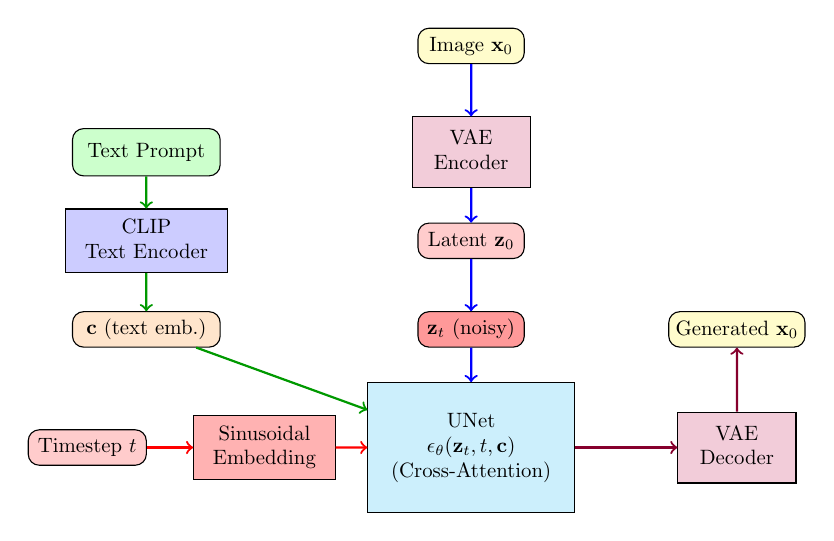
\begin{tikzpicture}[scale=0.75, every node/.style={scale=0.75}]

% Text Prompt
\node[draw, rounded corners, fill=green!20, minimum width=2.5cm, minimum height=0.8cm] (prompt) at (0,4) {Text Prompt};

% CLIP Text Encoder
\node[draw, rectangle, fill=blue!20, minimum width=2.5cm, minimum height=1cm] (clip) at (0,2.5) {\begin{tabular}{c}CLIP\\Text Encoder\end{tabular}};

% Text Embeddings
\node[draw, rounded corners, fill=orange!20, minimum width=2.5cm, minimum height=0.6cm] (emb) at (0,1) {$\mathbf{c}$ (text emb.)};

% Timestep
\node[draw, rounded corners, fill=red!20, minimum width=2cm, minimum height=0.6cm] (timestep) at (-1,-1) {Timestep $t$};

% Timestep Embedding
\node[draw, rectangle, fill=red!30, minimum width=2cm, minimum height=0.8cm] (time_emb) at (2,-1) {\begin{tabular}{c}Sinusoidal\\Embedding\end{tabular}};

% VAE Encoder
\node[draw, rectangle, fill=purple!20, minimum width=2cm, minimum height=1.2cm] (vae_enc) at (5.5,4) {\begin{tabular}{c}VAE\\Encoder\end{tabular}};

% Image
\node[draw, rounded corners, fill=yellow!20, minimum width=1.8cm, minimum height=0.6cm] (img) at (5.5,5.8) {Image $\mathbf{x}_0$};

% Latent
\node[draw, rounded corners, fill=red!20, minimum width=1.8cm, minimum height=0.6cm] (latent) at (5.5,2.5) {Latent $\mathbf{z}_0$};

% Noisy Latent
\node[draw, rounded corners, fill=red!40, minimum width=1.8cm, minimum height=0.6cm] (noisy_latent) at (5.5,1) {$\mathbf{z}_t$ (noisy)};

% UNet (center)
\node[draw, rectangle, fill=cyan!20, minimum width=3.5cm, minimum height=2.2cm] (unet) at (5.5,-1) {\begin{tabular}{c}UNet\\$\epsilon_\theta(\mathbf{z}_t, t, \mathbf{c})$\\(Cross-Attention)\end{tabular}};

% VAE Decoder
\node[draw, rectangle, fill=purple!20, minimum width=2cm, minimum height=1.2cm] (vae_dec) at (10,-1) {\begin{tabular}{c}VAE\\Decoder\end{tabular}};

% Generated Image
\node[draw, rounded corners, fill=yellow!20, minimum width=2cm, minimum height=0.6cm] (gen_img) at (10,1) {Generated $\mathbf{x}_0$};

% Arrows - Training path (blue)
\draw[->, thick, blue] (img) -- (vae_enc);
\draw[->, thick, blue] (vae_enc) -- (latent);
\draw[->, thick, blue] (latent) -- (noisy_latent);
\draw[->, thick, blue] (noisy_latent) -- (unet);

% Arrows - Text conditioning (green)
\draw[->, thick, green!60!black] (prompt) -- (clip);
\draw[->, thick, green!60!black] (clip) -- (emb);
\draw[->, thick, green!60!black] (emb) -- (unet);

% Arrows - Timestep conditioning (red)
\draw[->, thick, red] (timestep) -- (time_emb);
\draw[->, thick, red] (time_emb) -- (unet);

% Arrows - Generation path (purple)
\draw[->, thick, purple!70!black] (unet) -- (vae_dec);
\draw[->, thick, purple!70!black] (vae_dec) -- (gen_img);

\end{tikzpicture}
\end{center}

\vspace{0.3em}

{\small
\textbf{Training:} Compress to latents, add noise, learn $\epsilon_\theta(\mathbf{z}_t, t, \mathbf{c})$ to predict noise.

\textbf{Inference:} Start from $\mathbf{z}_T \sim \mathcal{N}(0,I)$, iteratively denoise guided by text and timestep.
}
\end{frame}




\begin{frame}{Why Stable Diffusion Works Better}

\begin{columns}

\column{0.5\textwidth}
\textbf{Pixel-Space Diffusion:}

\vspace{0.3cm}
\textcolor{red}{Disadvantages:}
\begin{itemize}
\item High dimensional (786,432D)
\item Slow training
\item Slow inference  
\item Expensive memory
\end{itemize}

\column{0.5\textwidth}
\textbf{Stable Diffusion:}

\vspace{0.3cm}
\textcolor{green!60!black}{Advantages:}
\begin{itemize}
\item Low dimensional (16,384D)
\item Fast training (48× faster)
\item Fast inference
\item Memory efficient
\item High quality via VAE
\end{itemize}

\end{columns}

\vspace{1em}

\begin{block}{Insight}
The VAE learns to compress images into a \alert{perceptually meaningful} latent space, discarding imperceptible details while preserving semantic information.
\end{block}

\end{frame}

\begin{frame}{Agenda}
\begin{itemize}
\item VAE: Compressing images to latent space.
  \vspace{0.7cm}
\item Text Conditioning with CLIP.
  \vspace{0.7cm}
\item Cross-Attention: Injecting text into UNet.
  \vspace{0.7cm}
\item Training Stable Diffusion.
  \vspace{0.7cm}
\item Inference and Sampling.
  \vspace{0.7cm}
\item Applications and fine-tuning.
\end{itemize}
\end{frame}


\begin{frame}{VAE: Compressing Images to Latent Space}
\textbf{Variational Autoencoder (VAE)} compresses images while preserving perceptual information.

\vspace{0.5em}
\textbf{Encoder $\phi$:} Maps image to latent distribution
\begin{equation*}
q_\phi(\mathbf{z}|\mathbf{x}) = \mathcal{N}(\mathbf{z}; \mu_\phi(\mathbf{x}), \sigma_\phi^2(\mathbf{x})I)
\end{equation*}
Sample latent: $\mathbf{z} = \mu_\phi(\mathbf{x}) + \sigma_\phi(\mathbf{x}) \odot \epsilon, \quad \epsilon \sim \mathcal{N}(0, I)$

\vspace{0.5em}
\textbf{Decoder $\psi$:} Reconstructs image from latent
\begin{equation*}
p_\psi(\mathbf{x}|\mathbf{z}) = \mathcal{N}(\mathbf{x}; \mu_\psi(\mathbf{z}), I)
\end{equation*}

\vspace{0.5em}
\textbf{Training objective (negative ELBO - Evidence Lower Bound):}
\begin{equation*}
\mathcal{L}_{\text{VAE}} = \underbrace{\|\mathbf{x} - \hat{\mathbf{x}}\|^2}_{\text{reconstruction}} + \underbrace{\beta \cdot \text{KL}(q_\phi(\mathbf{z}|\mathbf{x}) \| p(\mathbf{z}))}_{\text{regularization}}
\end{equation*}
where $p(\mathbf{z}) = \mathcal{N}(0, I)$ and $\beta$ controls the trade-off.
\end{frame}

\begin{frame}{VAE Architecture for Stable Diffusion}

\textbf{Scaling factor:} Latents are scaled by $s = 0.18215$ for numerical stability.

\vspace{0.5em}

\textbf{Encoder:} $\phi: \mathbb{R}^{512 \times 512 \times 3} \to \mathbb{R}^{64 \times 64 \times 4}$

\begin{itemize}
\item Downsampling factor: $8\times$ in spatial dimensions.
\item Compression ratio: $48\times$ (from 786,432 to 16,384 dimensions).
\item Architecture: Convolutional layers with residual blocks.
\end{itemize}

\vspace{0.2em}

\textbf{Encoding process:}
\begin{align*}
\mathbf{x} &\in [-1, 1]^{512 \times 512 \times 3} \quad \text{(normalized image)}. \\
\mathbf{x'} &= \phi(\mathbf{x}) \in \mathbb{R}^{64 \times 64 \times 4}. \\
[\mu_\phi(\mathbf{x}), \log \sigma^2_\phi(x)] &\leftarrow [Linear(\mathbf{x'}),Linear(\mathbf{x'})]\\
\mathbf{z} & \leftarrow s \cdot [\mu_\phi(\mathbf{x}) + \sigma_\phi(\mathbf{x}) \odot \epsilon] \quad \text{(for diffusion)}.
\end{align*}

\vspace{0.2em}

\textbf{Decoder:} $\psi: \mathbb{R}^{64 \times 64 \times 4} \to \mathbb{R}^{512 \times 512 \times 3}$

\begin{equation*}
\hat{\mathbf{x}} = \psi(\mathbf{z}/s) \in [-1, 1]^{512 \times 512 \times 3}.
\end{equation*}

\end{frame}

\begin{frame}{VAE Properties}

\textbf{Properties that make VAE suitable for diffusion:}

\vspace{0.5em}

\begin{enumerate}
\item \textbf{Perceptual compression:}
\begin{itemize}
    \item Removes imperceptible high-frequency details.
    \item Preserves semantic and structural information.
    \item Low reconstruction error: $\|\mathbf{x} - \hat{\mathbf{x}}\|^2 < 0.01$
      .
\end{itemize}

\vspace{0.3em}

\item \textbf{Smooth latent space:}
\begin{itemize}
    \item Similar images map to nearby latents.
    \item Enables smooth interpolation.
    \item Suitable for Gaussian diffusion.
\end{itemize}

\vspace{0.3em}

\item \textbf{Computational efficiency:}
\begin{itemize}
    \item $48\times$ fewer dimensions than pixels.
    \item Faster forward/backward passes in UNet.
    \item Lower memory requirements.
\end{itemize}
\end{enumerate}

\vspace{0.5em}

\textbf{Trade-off:} Slight loss of fine details (assuming large training set) vs. massive speedup.

\end{frame}

\begin{frame}{Text Conditioning with CLIP}

\textbf{CLIP (Contrastive Language-Image Pre-training)} encodes text into semantic embeddings.

\vspace{0.5em}

\textbf{Architecture:} Transformer-based text encoder, pre-trained on 400M image-text pairs, maps text to fixed-dimensional space: $\mathbb{R}^{77 \times 768}$.


\vspace{0.5em}

\textbf{Text encoding process:}

\begin{align*}
\text{text} &\xrightarrow{\text{Tokenizer}} [t_1, t_2, \ldots, t_{77}] \in \mathbb{N}^{77} \\
[t_1, \ldots, t_{77}] &\xrightarrow{\text{Embedding}} [\mathbf{e}_1, \ldots, \mathbf{e}_{77}] \in \mathbb{R}^{77 \times 768} \\
[\mathbf{e}_1, \ldots, \mathbf{e}_{77}] &\xrightarrow{\text{Transformer}} \mathbf{c} \in \mathbb{R}^{77 \times 768}
\end{align*}

\textbf{Properties:}
\begin{itemize}
\item Maximum sequence length: 77 tokens.
\item Padding/truncation for variable-length prompts.
\item Similar meanings $\Rightarrow$ similar embeddings.
\end{itemize}

\end{frame}

\begin{frame}{Classifier-Free Guidance}

\textbf{Problem:} How to control the strength of text conditioning?

\vspace{0.3em}

\textbf{Solution:} Classifier-Free Guidance (CFG) - interpolate between conditional and unconditional predictions.

\vspace{0.5em}

\textbf{Training:} Randomly drop text conditioning ($p = 0.1$)
\begin{equation*}
\epsilon_\theta(\mathbf{z}_t, t, \mathbf{c}) \quad \text{and} \quad \epsilon_\theta(\mathbf{z}_t, t, \emptyset)
\end{equation*}

\vspace{0.3em}

\textbf{Inference:} Combine both predictions
\begin{equation*}
\tilde{\epsilon}_\theta = \underbrace{\epsilon_\theta(\mathbf{z}_t, t, \emptyset)}_{\text{unconditional}} + w \cdot \underbrace{(\epsilon_\theta(\mathbf{z}_t, t, \mathbf{c}) - \epsilon_\theta(\mathbf{z}_t, t, \emptyset))}_{\text{guidance direction}}
\end{equation*}
where $w > 0$ is the \alert{guidance scale}.

\vspace{0.1em}

\textbf{Effects of guidance scale:}
\begin{itemize}
\item $w = 1$: Standard conditional generation.
\item $w > 1$: Stronger adherence to prompt (typical: $w = 7.5$).
\item $w < 1$: Weaker conditioning, more creative.
\end{itemize}
\end{frame}

\begin{frame}{UNet with Cross-Attention}

\textbf{Modified ResBlock with cross-attention:}

\vspace{0.3em}

\begin{align*}
\mathbf{h}^{(0)} &= \text{ResBlock}(\mathbf{z}_t, \mathbf{e}_t) \quad \text{(spatial conv + time embed)} \\
\mathbf{h}^{(1)} &= \text{SelfAttn}(\mathbf{h}^{(0)}) + \mathbf{h}^{(0)} \quad \text{(self-attention)} \\
\mathbf{h}^{(2)} &= \text{CrossAttn}(\mathbf{h}^{(1)}, \mathbf{c}) + \mathbf{h}^{(1)} \quad \text{(text conditioning)} \\
\mathbf{h}^{(3)} &= \text{FFN}(\mathbf{h}^{(2)}) + \mathbf{h}^{(2)} \quad \text{(feed-forward)}
\end{align*}

\vspace{0.5em}

\textbf{Three inputs to UNet:}
\begin{enumerate}
\item $\mathbf{z}_t$: Noisy latent at timestep $t$.
\item $t$: Timestep (via sinusoidal embedding $\mathbf{e}_t$).
\item $\mathbf{c}$: Text embeddings from CLIP.
\end{enumerate}

\vspace{0.5em}

\textbf{Output:} Predicted noise $\epsilon_\theta(\mathbf{z}_t, t, \mathbf{c})$.

\vspace{0.5em}

\textbf{Key:} Apply attention only at \alert{lower resolutions} ($\leq$ 32 $\times$ 32 pixels).
\end{frame}

\begin{frame}{Attention Mechanism: Core Concept}
\textbf{Goal:} Allow each position to attend to relevant information.

\vspace{0.5em}
\textbf{Single-Head Attention:}
\begin{align*}
\mathbf{Q} &= \mathbf{Z} \mathbf{W}_Q \in \mathbb{R}^{n \times d_k} \quad \text{(queries)} \\
\mathbf{K} &= \mathbf{Z} \mathbf{W}_K \in \mathbb{R}^{n \times d_k} \quad \text{(keys)} \\
\mathbf{V} &= \mathbf{Z} \mathbf{W}_V \in \mathbb{R}^{n \times d_v} \quad \text{(values)}
\end{align*}
\small Typically: $d_k = d_v$.

\begin{equation*}
\text{Attention}(\mathbf{Q}, \mathbf{K}, \mathbf{V}) = \text{softmax}\left(\frac{\mathbf{Q}\mathbf{K}^T}{\sqrt{d_k}}\right)\mathbf{V}
\end{equation*}

\vspace{0.1em}
\begin{itemize}
\item $\mathbf{Q}\mathbf{K}^T \in \mathbb{R}^{n \times n}$: attention scores (who attends to whom).
\item Softmax: normalize scores to probabilities.
\item Multiply by $\mathbf{V}$: weighted combination of values.
\end{itemize}

\textbf{Limitation:} Single attention pattern solved by
\alert{multiple attention heads}.
\end{frame}

\begin{frame}{Multi-Head Attention}
Run $h$ attention operations in parallel (different ``heads'').

\textbf{For each head $i = 1, \ldots, h$:}
\begin{enumerate}
\item \textbf{Project to head $i$} using independent $\mathbf{W}_Q^i, \mathbf{W}_K^i, \mathbf{W}_V^i$.
\begin{align*}
\mathbf{Q}_i &= \mathbf{Z} \mathbf{W}_Q^i \in \mathbb{R}^{n \times d_k} \\
\mathbf{K}_i &= \mathbf{Z} \mathbf{W}_K^i \in \mathbb{R}^{n \times d_k} \\
\mathbf{V}_i &= \mathbf{Z} \mathbf{W}_V^i \in \mathbb{R}^{n \times d_v}
\end{align*}

\item \textbf{Compute attention:}
\begin{equation*}
\text{head}_i = \text{softmax}\left(\frac{\mathbf{Q}_i\mathbf{K}_i^T}{\sqrt{d_k}}\right)\mathbf{V}_i \in \mathbb{R}^{n \times d_v}
\end{equation*}
\end{enumerate}

\textbf{Combine all heads:}
\begin{equation*}
\text{MultiHead}(\mathbf{Z}) = \text{Concat}(\text{head}_1, \ldots, \text{head}_h) \mathbf{W}^O \in \mathbb{R}^{n \times d}
\end{equation*}
where $\mathbf{W}^O \in \mathbb{R}^{(h \cdot d_v) \times d}$ mixes information across heads - e.g., $d_k = d_v = d/h$ so concatenation gives \alert{dimension $d$} (from the model.
\end{frame}

\begin{frame}{Self-Attention in UNet: Spatial Coherence}
\textbf{Goal:} Allow spatial locations (pixels) to attend to each other.

\vspace{0.5em}
\textbf{Self-Attention:} Q, K, V all come from the same source $\mathbf{Z}$.
\begin{align*}
\mathbf{Q}_i &= \mathbf{Z} \mathbf{W}_Q^i \in \mathbb{R}^{(H \cdot W) \times d_k} \quad \text{(queries from latents)} \\
\mathbf{K}_i &= \mathbf{Z} \mathbf{W}_K^i \in \mathbb{R}^{(H \cdot W) \times d_k} \quad \text{(keys from latents)} \\
\mathbf{V}_i &= \mathbf{Z} \mathbf{W}_V^i \in \mathbb{R}^{(H \cdot W) \times d_v} \quad \text{(values from latents)}
\end{align*}

where $\mathbf{Z} \in \mathbb{R}^{(H \cdot W) \times d}$ are flattened UNet features.

\vspace{0.2em}
\textbf{Each head $i$:}
\begin{equation*}
\text{head}_i = \text{softmax}\left(\frac{\mathbf{Q}_i\mathbf{K}_i^T}{\sqrt{d_k}}\right)\mathbf{V}_i \in \mathbb{R}^{(H \cdot W) \times d_v}
\end{equation*}

\textbf{Output:} $\text{Concat}(\text{head}_1, \ldots, \text{head}_h) \mathbf{W}^O \in \mathbb{R}^{(H \cdot W) \times d}$

\vspace{0.3em}
\textbf{Key:} $\mathbf{Q}_i\mathbf{K}_i^T \in \mathbb{R}^{(H \cdot W) \times (H \cdot W)}$ — each pixel attends to \alert{all pixels}!
\end{frame}

\begin{frame}{Cross-Attention in UNet: Text Conditioning}
\textbf{Goal:} Condition each spatial location on the text prompt.

\vspace{0.5em}
\textbf{Cross-Attention:} Q from latents, K,V from text.
\begin{align*}
\mathbf{Q}_i &= \mathbf{Z} \mathbf{W}_Q^i \in \mathbb{R}^{(H \cdot W) \times d_k} \quad \text{(queries from latents)} \\
\mathbf{K}_i &= \mathbf{C} \mathbf{W}_K^i \in \mathbb{R}^{77 \times d_k} \quad \text{(keys from text)} \\
\mathbf{V}_i &= \mathbf{C} \mathbf{W}_V^i \in \mathbb{R}^{77 \times d_v} \quad \text{(values from text)}
\end{align*}

where $\mathbf{Z} \in \mathbb{R}^{(H \cdot W) \times d}$ (UNet), $\mathbf{C} \in \mathbb{R}^{77 \times 768}$ (CLIP text).

\vspace{0.3em}
\textbf{Each head $i$:}
\begin{equation*}
\text{head}_i = \text{softmax}\left(\frac{\mathbf{Q}_i\mathbf{K}_i^T}{\sqrt{d_k}}\right)\mathbf{V}_i \in \mathbb{R}^{(H \cdot W) \times d_v}
\end{equation*}

\textbf{Output:} $\text{Concat}(\text{head}_1, \ldots, \text{head}_h) \mathbf{W}^O \in \mathbb{R}^{(H \cdot W) \times d}$

\vspace{0.4em}
\textbf{Key:} $\mathbf{Q}_i\mathbf{K}_i^T \in \mathbb{R}^{(H \cdot W) \times 77}$ — each pixel attends to \alert{text tokens}!
\end{frame}

\begin{frame}{Implementation Note: Efficient Multi-Head Attention}
\textbf{Conceptual:} $h$ independent projections $\mathbf{W}_Q^1, \ldots, \mathbf{W}_Q^h$.

\textbf{Efficient implementation:} Combine into single large matrix.
\begin{equation*}
\mathbf{W}_Q = \begin{bmatrix} \mathbf{W}_Q^1 & \mathbf{W}_Q^2 & \cdots & \mathbf{W}_Q^h \end{bmatrix} \in \mathbb{R}^{d \times (h \cdot d_k)}
\end{equation*}

\textbf{Steps:}
\begin{enumerate}
\item \textbf{Single projection:} $\mathbf{Q} = \mathbf{Z} \mathbf{W}_Q \in \mathbb{R}^{n \times (h \cdot d_k)}$.
\item \textbf{Reshape:} Split last dimension into heads: $\mathbb{R}^{n \times h \times d_k}$.
\item \textbf{Transpose:} $\mathbb{R}^{h \times n \times d_k}$ for parallel computation.
\item \textbf{Attention:} Compute $h$ attentions in parallel (batched).
\item \textbf{Concatenate:} Reshape back to $\mathbb{R}^{n \times (h \cdot d_k)}$.
\item \textbf{Output projection:} $\mathbf{W}^O$.
\end{enumerate}

\vspace{0.3em}
\textbf{Result:} Mathematically equivalent, computationally efficient in GPUs!
\end{frame}


\begin{frame}{Training Stable Diffusion}

\textbf{Training objective:} Learn to predict noise in latent space.

\vspace{0.5em}

\textbf{Loss function:}
\begin{equation*}
\mathcal{L} = \mathbb{E}_{\mathbf{z}_0, \mathbf{c}, \epsilon, t}\left[\|\epsilon - \epsilon_\theta(\mathbf{z}_t, t, \mathbf{c})\|^2\right]
\end{equation*}

where:
\begin{itemize}
\item $\mathbf{z}_0 = \phi(\mathbf{x}_0)$: Encoded latent from image.
\item $\mathbf{c} = \text{CLIP}(\text{prompt})$: Text embedding.
\item $t \sim \text{Uniform}(1, T)$: Random timestep.
\item $\epsilon \sim \mathcal{N}(0, I)$: Random noise.
\item $\mathbf{z}_t = \sqrt{\bar{\alpha}_t}\mathbf{z}_0 + \sqrt{1-\bar{\alpha}_t}\epsilon$: Noisy latent.
\end{itemize}

\vspace{0.5em}

\textbf{Frozen components:}
\begin{itemize}
\item VAE encoder and decoder.
\item CLIP text encoder.
\end{itemize}

\textbf{Trainable component:}
\begin{itemize}
\item UNet denoising network only.
\end{itemize}

\end{frame}

\begin{frame}{Training Algorithm}

  \begin{algorithm}[H]
    \tiny
\caption{Training Stable Diffusion}
\begin{algorithmic}[1]
\REQUIRE Dataset of image-text pairs $\{(\mathbf{x}^{(i)}, \text{prompt}^{(i)})\}$, VAE encoder $\phi$, CLIP text encoder, UNet $\epsilon_\theta$.
\STATE Freeze VAE and CLIP text encoders.
\REPEAT
    \STATE Sample batch $\{(\mathbf{x}^{(i)}, \text{prompt}^{(i)})\}_{i=1}^B$.
    \STATE \textbf{// Encode to latent space}.
    \STATE $\mathbf{z}_0^{(i)} \leftarrow s \cdot \phi(\mathbf{x}^{(i)})$ for all $i$ \COMMENT{VAE encoding}.
    \STATE \textbf{// Encode text prompts}.
    \STATE $\mathbf{c}^{(i)} \leftarrow \text{CLIP}(\text{prompt}^{(i)})$ for all $i$ \COMMENT{Text encoding}.
    \STATE \textbf{// Randomly drop conditioning (10\% of samples)}.
    \STATE With probability 0.1: $\mathbf{c}^{(i)} \leftarrow \emptyset$ \COMMENT{For CFG}.
    \STATE \textbf{// Sample random timesteps and noise}.
    \STATE Sample $t^{(i)} \sim \text{Uniform}(\{1, \ldots, T\})$ for all $i$.
    \STATE Sample $\epsilon^{(i)} \sim \mathcal{N}(0, I)$ for all $i$.
    \STATE \textbf{// Add noise to latents}.
    \STATE $\mathbf{z}_t^{(i)} \leftarrow \sqrt{\bar{\alpha}_{t^{(i)}}}\mathbf{z}_0^{(i)} + \sqrt{1-\bar{\alpha}_{t^{(i)}}}\epsilon^{(i)}$.
    \STATE \textbf{// Predict noise}.
    \STATE $\hat{\epsilon}^{(i)} \leftarrow \epsilon_\theta(\mathbf{z}_t^{(i)}, t^{(i)}, \mathbf{c}^{(i)})$ \COMMENT{UNet forward}.
    \STATE \textbf{// Compute loss and update}.
    \STATE $\mathcal{L} \leftarrow \frac{1}{B}\sum_{i=1}^B \|\epsilon^{(i)} - \hat{\epsilon}^{(i)}\|^2$.
    \STATE Update $\theta$ using $\nabla_\theta \mathcal{L}$.
\UNTIL{converged.}
\end{algorithmic}
\end{algorithm}

\end{frame}

\begin{frame}{Sampling Algorithm (Inference)}

  \begin{algorithm}[H]
    \tiny
\caption{Sampling from Stable Diffusion}
\begin{algorithmic}[1]
\REQUIRE Trained UNet $\epsilon_\theta$, VAE decoder $\psi$, CLIP text encoder, text prompt, guidance scale $w$
\STATE \textbf{// Encode text prompt}
\STATE $\mathbf{c} \leftarrow \text{CLIP}(\text{prompt})$ \COMMENT{Conditional embedding}
\STATE $\mathbf{c}_\emptyset \leftarrow \text{CLIP}(\text{``''})$ \COMMENT{Unconditional (empty) embedding}
\STATE \textbf{// Start from random noise}
\STATE Sample $\mathbf{z}_T \sim \mathcal{N}(0, I)$ \COMMENT{Pure noise in latent space}
\STATE \textbf{// Denoising loop}
\FOR{$t = T, T-1, \ldots, 1$}
    \STATE \textbf{// Predict noise with and without conditioning}
    \STATE $\epsilon_{\text{uncond}} \leftarrow \epsilon_\theta(\mathbf{z}_t, t, \mathbf{c}_\emptyset)$
    \STATE $\epsilon_{\text{cond}} \leftarrow \epsilon_\theta(\mathbf{z}_t, t, \mathbf{c})$
    \STATE \textbf{// Apply classifier-free guidance}
    \STATE $\hat{\epsilon} \leftarrow \epsilon_{\text{uncond}} + w \cdot (\epsilon_{\text{cond}} - \epsilon_{\text{uncond}})$
    \STATE \textbf{// Denoise one step}
    \STATE $\mathbf{z}_{t-1} \leftarrow \text{scheduler.step}(\hat{\epsilon}, t, \mathbf{z}_t)$
\ENDFOR
\STATE \textbf{// Decode to image}
\STATE $\mathbf{x}_0 \leftarrow \psi(\mathbf{z}_0 / s)$ \COMMENT{VAE decoding}
\STATE \textbf{return} $\mathbf{x}_0$
\end{algorithmic}
\end{algorithm}

\end{frame}

\begin{frame}{Inference: Visual Demonstration}

\textbf{Text-to-Image Generation} (\alert{see code1-stable-diffusion.py})

\vspace{0.3em}

Prompt: \textit{``a running dog''}

\begin{center}
\includegraphics[width=0.9\textwidth]{./figs/stable_diffusion_results.png}
\end{center}

\vspace{0.3em}

\textbf{Left:} Original image for reference.

\textbf{Center:} Text-to-image (from pure noise).

\textbf{Right:} Image-to-image (original + noise, then denoise with text guidance).

\end{frame}

\begin{frame}{Image-to-Image Generation}

Start from a noisy version of an existing image to preserve its
structure rather than generating a new image from pure noise.

\vspace{0.5em}

\textbf{Process:}

\begin{enumerate}
\item Encode source image: $\mathbf{z}_0 = \phi(\mathbf{x}_{\text{source}})$.

\vspace{0.3em}

\item Add controlled noise: 
\begin{equation*}
\mathbf{z}_{t_0} = \sqrt{\bar{\alpha}_{t_0}}\mathbf{z}_0 + \sqrt{1-\bar{\alpha}_{t_0}}\epsilon
\end{equation*}

\vspace{0.3em}

\item Denoise from $t_0$ to $0$ (instead of $T$ to $0$).

\vspace{0.3em}

\item Decode: $\mathbf{x}_{\text{output}} = \psi(\mathbf{z}_0)$.
\end{enumerate}

\vspace{0.5em}

\textbf{Strength parameter $s \in [0, 1]$, $t_0 = s \cdot T$.}
\begin{itemize}
\item $s = 0$: No change (skip denoising).
\item $s = 0.3$: Subtle modifications, preserves image structure.
\item $s = 0.7$: Major changes, follows prompt more.
\item $s = 1.0$: Equivalent to text-to-image.
\end{itemize}

\end{frame}

\begin{frame}{Applications of Stable Diffusion}

\begin{enumerate}
\item \textbf{Text-to-Image:} Generate images from text descriptions (e.g., art generation).

\vspace{0.5cm}

\item \textbf{Image-to-Image:} Transform existing images (e.g., style
  transfer).

\vspace{0.5cm}

\item \textbf{Inpainting:} Fill masked regions (e.g., object removal, image completion).

\vspace{0.5cm}

\item \textbf{Super-resolution:} Upscale low-res images (e.g., detail enhancement, quality improvement).
\end{enumerate}

\end{frame}

\begin{frame}{Fine-tuning Stable Diffusion}

\textbf{Why fine-tune?}
\begin{itemize}
\item Adapt to specific domains (e.g., medical images, art styles).
\item Learn new concepts or objects.
\item Improve quality on specific types of prompts.
\end{itemize}

\vspace{0.5em}

\textbf{Full Fine-tuning:}
\begin{itemize}
\item Train entire UNet on custom dataset.
\item Requires: Many images (1000+), high compute (GPU days).
\item Best quality but expensive.
\end{itemize}

\vspace{0.5em}

\textbf{Efficient Alternative: LoRA (Low-Rank Adaptation).}
\begin{itemize}
\item Freeze original weights, add small trainable layers.
\item Requires: Few images (10-100), low compute (GPU hours).
\item Good quality with minimal resources.
\end{itemize}

\vspace{0.5em}

\alert{Let's understand LoRA...}

\end{frame}

\begin{frame}{LoRA: Low-Rank Adaptation}

Instead of updating all weights $\mathbf{W} \in \mathbb{R}^{d \times
  k}$, add a low-rank perturbation.

\vspace{0.1em}

\textbf{Original layer:}
\begin{equation*}
\mathbf{y} = \mathbf{W}\mathbf{x}
\end{equation*}

\textbf{LoRA layer:}
\begin{equation*}
\mathbf{y} = \underbrace{\mathbf{W}}_{\text{frozen}}\mathbf{x} + \underbrace{\mathbf{B}\mathbf{A}}_{\text{trainable}}\mathbf{x}
\end{equation*}

where:
\begin{itemize}
\item $\mathbf{W} \in \mathbb{R}^{d \times k}$: Original frozen weights.
\item $\mathbf{B} \in \mathbb{R}^{d \times r}$, $\mathbf{A} \in \mathbb{R}^{r \times k}$: Trainable low-rank matrices.
\item $r \ll \min(d, k)$: Rank (typically $r = 4, 8, 16$).
\end{itemize}

\vspace{0.1em}

\textbf{Parameter reduction:}
\begin{equation*}
\text{Original: } d \times k \quad \Rightarrow \quad \text{LoRA: } r(d + k)
\end{equation*}

Ex: $d=k=1024$, $r=8$: $1,048,576 \Rightarrow 16,384$ (64× reduction!).

\end{frame}

\begin{frame}{LoRA: Low-Rank Adaptation}

\textbf{Intrinsic Dimensionality Hypothesis:}

It works when the updates to weights during fine-tuning lies in a
low-dimensional subspace.

\vspace{0.2em}

\textbf{Mathematical intuition:}

Full update: $\mathbf{W}_{\text{new}} = \mathbf{W} + \Delta\mathbf{W}$

LoRA approximation: $\Delta\mathbf{W} \approx \mathbf{B}\mathbf{A}$ where $\text{rank}(\mathbf{B}\mathbf{A}) = r$

\vspace{0.2em}

\textbf{Benefits for Stable Diffusion fine-tuning:}

\begin{enumerate}
\item \textbf{Memory efficient:} Only train $\sim$1\% of parameters.
\vspace{0.2cm}
\item \textbf{Fast training:} Fewer parameters to update.
\vspace{0.2cm}
\item \textbf{Modular:} Can swap LoRA weights without changing base model.
\vspace{0.2cm}
\item \textbf{Composable:} Can combine multiple LoRAs.
\vspace{0.2cm}
\item \textbf{No catastrophic forgetting:} Base model stays intact.
\end{enumerate}

\vspace{0.2em}

\textbf{Where to apply LoRA:} Attention projection layers in UNet.

\end{frame}

\begin{frame}{Fine-tuning: Training Setup}

\textbf{\alert{Full fine-tuning}} (\alert{see code2-finetune-stable-model.py}):

\vspace{0.3em}

\textbf{Frozen components:}
\begin{itemize}
\item VAE encoder/decoder.
\item CLIP text encoder.
\end{itemize}

\textbf{Trainable:}
\begin{itemize}
\item Entire UNet (or with LoRA: only LoRA layers).
\end{itemize}

\vspace{0.5em}

\textbf{Training hyperparameters:}
\begin{itemize}
\item Learning rate: $1 \times 10^{-5}$ (lower than pretraining).
\item Batch size: 1-4 (limited by GPU memory).
\item Resolution: 384×384 or 512×512.
\item Epochs: 10-100 (depends on dataset size).
\end{itemize}

\vspace{0.3em}

\textbf{Memory optimizations:}
\begin{itemize}
\item Gradient checkpointing (trades compute for memory).
\item 8-bit optimizer (50\% memory reduction).
\item Mixed precision training (FP16).
\end{itemize}

\end{frame}

\begin{frame}{Fine-tuning Algorithm}

  \begin{algorithm}[H]
    \tiny
\caption{Fine-tuning Stable Diffusion (Full or LoRA)}
\begin{algorithmic}[1]
\REQUIRE Custom dataset $\{(\mathbf{x}^{(i)}, \text{prompt}^{(i)})\}$, pretrained model
\STATE Load pretrained VAE, CLIP, UNet
\STATE Freeze VAE and CLIP
\IF{using LoRA}
    \STATE Freeze UNet base weights
    \STATE Add LoRA layers to attention projections
    \STATE Initialize $\mathbf{A} \sim \mathcal{N}(0, \sigma^2)$, $\mathbf{B} = \mathbf{0}$
\ENDIF
\REPEAT
    \STATE Sample batch $\{(\mathbf{x}^{(i)}, \text{prompt}^{(i)})\}$
    \STATE Encode: $\mathbf{z}_0^{(i)} \leftarrow \mathcal{E}(\mathbf{x}^{(i)})$, $\mathbf{c}^{(i)} \leftarrow \text{CLIP}(\text{prompt}^{(i)})$
    \STATE Sample $t^{(i)}$, $\epsilon^{(i)}$
    \STATE Compute $\mathbf{z}_t^{(i)} = \sqrt{\bar{\alpha}_{t^{(i)}}}\mathbf{z}_0^{(i)} + \sqrt{1-\bar{\alpha}_{t^{(i)}}}\epsilon^{(i)}$
    \STATE Predict: $\hat{\epsilon}^{(i)} \leftarrow \epsilon_\theta(\mathbf{z}_t^{(i)}, t^{(i)}, \mathbf{c}^{(i)})$
    \STATE Loss: $\mathcal{L} = \frac{1}{B}\sum_{i} \|\epsilon^{(i)} - \hat{\epsilon}^{(i)}\|^2$
    \IF{using LoRA}
        \STATE Update only LoRA weights ($\mathbf{A}$, $\mathbf{B}$)
    \ELSE
        \STATE Update all UNet weights
    \ENDIF
\UNTIL{converged}
\STATE Save fine-tuned model (or LoRA weights)
\end{algorithmic}
\end{algorithm}

\end{frame}

\begin{frame}{Fine-tuned Model Inference}

\textbf{Inference with fine-tuned model}.

\vspace{0.5em}

\textbf{Process:}
\begin{enumerate}
\item Load pretrained VAE and CLIP (unchanged).
\item Load fine-tuned UNet (or base UNet + LoRA weights).
\item Generate images using standard sampling algorithm.
\end{enumerate}

\vspace{0.5em}

\textbf{Example prompt:} \textit{``a jumping dog with sunglasses wearing a bear hat''}

\begin{center}
\includegraphics[scale=0.2]{./figs/generated_20251019_171943.png}
\end{center}

{\small \textit{(Image generated using \alert{code3-stable-model-inference.py} with user prompt)}}

\end{frame}

\begin{frame}{What We Learned}

\begin{enumerate}
\item \textbf{Stable Diffusion = Latent Diffusion + Text Conditioning}
\begin{itemize}
    \item VAE compresses to $48\times$ smaller latent space.
    \item Diffusion operates in latent space (much faster).
\end{itemize}

\vspace{0.3cm}

\item \textbf{Three key components:}
\begin{itemize}
    \item VAE: Compression and reconstruction.
    \item CLIP: Text understanding.
    \item UNet: Denoising with cross-attention.
\end{itemize}

\vspace{0.3cm}

\item \textbf{Training:} Predict noise in latent space conditioned on text.

\vspace{0.3cm}

\item \textbf{Inference:} Iterative denoising with classifier-free guidance.

\vspace{0.3cm}

\item \textbf{Fine-tuning:} Adapt to custom domains.
\begin{itemize}
    \item Full: High quality, high cost.
    \item LoRA: Good quality, low cost (recommended).
\end{itemize}
\end{enumerate}

\vspace{0.5em}

\textbf{See also other techniques:} DreamBooth, IP-Adapter, Textual
Inversion, and ControlNet.

\end{frame}

\begin{frame}{Take-home Message}
  \begin{itemize}
  \item VAE (see \alert{code4-train-vae.py}) requires several
    thousands of samples at least to reduce blurring and generate
    clear images in stable diffusion.
    \vspace{0.5cm}
  \item Training a simple diffusion model from scratch also requires
    many samples (\alert{code5-train-diffusion-from-scratch.py}), but
    stable diffusion can considerably amend the problem
    (\alert{code5-train-stable-diffusion-from-scratch.py}).
    \vspace{0.5cm}
  \item Real life problems may present a few images from domain
    difficult to adapt the model via fine-tuning.
    \vspace{0.5cm}
  \item LoRA is an alternative (\alert{code6-train-model-with-lora.py}
    and \alert{code7-generate-image-with-lora.py}), but

    \vspace{0.5cm} \textbf{can it adapt a pretrained stable diffusion
      model to a distinct domain with a few images?}
  \end{itemize}
\end{frame}

\end{document}
